% ========================================
%	Header einbinden
% ========================================

\documentclass[bibtotoc,titlepage]{scrartcl}

% Deutsche Spracheinstellungen
\usepackage[ngerman,german]{babel, varioref}
\usepackage[T1]{fontenc}
\usepackage[utf8]{inputenc}

%\usepackage{marvosym}

\usepackage{amsfonts}
\usepackage{amssymb}
\usepackage{amsmath}
\usepackage{amscd}
\usepackage{amstext}

\usepackage{longtable}

%\usepackage{bibgerm}

\usepackage{footnpag}

\usepackage{ifthen}                 %%% package for conditionals in TeX
\usepackage[amssymb]{SIunits}
%Für textumflossene Bilder und Tablellen
%\usepackage{floatflt} - veraltet

%Für Testzwecke aktivieren, zeigt labels und refs im Text an.
%\usepackage{showkeys}

% Abstand zwischen zwei Absätzen nach DIN (1,5 Zeilen)
% \setlength{\parskip}{1.5ex plus0.5ex minus0.5ex}

% Einrückung am Anfang eines neuen Absatzes nach DIN (keine)
%\setlength{\parindent}{0pt}

% Ränder definieren
% \setlength{\oddsidemargin}{0.3cm}
% \setlength{\textwidth}{15.6cm}

% bessere Bildunterschriften
%\usepackage[center]{caption2}


% Problemlösungen beim Umgang mit Gleitumgebungen
\usepackage{float}

% Nummeriert bis zur Strukturstufe 3 (also <section>, <subsection> und <subsubsection>)
%\setcounter{secnumdepth}{3}

% Führt das Inhaltsverzeichnis bis zur Strukturstufe 3
%\setcounter{tocdepth}{3}
\usepackage[version=3]{mhchem}
	\mhchemoptions{minus-sidebearing-left=0.06em, minus-sidebearing-right=0.11em}
\usepackage{exscale}

\newenvironment{dsm} {\begin{displaymath}} {\end{displaymath}}
\newenvironment{vars} {\begin{center}\scriptsize} {\normalsize \end{center}}


\newcommand {\en} {\varepsilon_0}               % Epsilon-Null aus der Elektrodynamik
\newcommand {\lap} {\; \mathbf{\Delta}}         % Laplace-Operator
\newcommand {\R} { \mathbb{R} }                 % Menge der reellen Zahlen
\newcommand {\e} { \ \mathbf{e} }               % Eulersche Zahl
\renewcommand {\i} { \mathbf{i} }               % komplexe Zahl i
\newcommand {\N} { \mathbb{N} }                 % Menge der nat. Zahlen
\newcommand {\C} { \mathbb{C} }                 % Menge der kompl. Zahlen
\newcommand {\Z} { \mathbb{Z} }                 % Menge der kompl. Zahlen
\newcommand {\limi}[1]{\lim_{#1 \rightarrow \infty}} % Limes unendlich
\newcommand {\sumi}[1]{\sum_{#1=0}^\infty}
\newcommand {\rot} {\; \mathrm{rot} \,}         % Rotation
\newcommand {\grad} {\; \mathrm{grad} \,}       % Gradient
\newcommand {\dive} {\; \mathrm{div} \,}        % Divergenz
\newcommand {\dx} {\; \mathrm{d} }              % Differential d
\newcommand {\cotanh} {\; \mathrm{cotanh} \,}   %Cotangenshyperbolicus
\newcommand {\asinh} {\; \mathrm{areasinh} \,}  %Area-Sinus-Hyp.
\newcommand {\acosh} {\; \mathrm{areacosh} \,}  %Area-Cosinus-H.
\newcommand {\atanh} {\; \mathrm{areatanh} \,}  %Area Tangens-H.
\newcommand {\acoth} {\; \mathrm{areacoth} \,}  % Area-cotangens
\newcommand {\Sp} {\; \mathrm{Sp} \,}
\newcommand {\mbe} {\stackrel{\text{!}}{=}}     %Must Be Equal
\newcommand{\qed} { \hfill $\square$\\}
\renewcommand{\i} {\imath}
\def\captionsngerman{\def\figurename{\textbf{Abb.}}}

%%%%%%%%%%%%%%%%%%%%%%%%%%%%%%%%%%%%%%%%%%%%%%%%%%%%%%%%%%%%%%%%%%%%%%%%%%%%
% SWITCH FOR PDFLATEX or LATEX
%%%%%%%%%%%%%%%%%%%%%%%%%%%%%%%%%%%%%%%%%%%%%%%%%%%%%%%%%%%%%%%%%%%%%%%%%%%%
%%%
\ifx\pdfoutput\undefined %%%%%%%%%%%%%%%%%%%%%%%%%%%%%%%%%%%%%%%%% LATEX %%%
%%%
\usepackage[dvips]{graphicx}       %%% graphics for dvips
\DeclareGraphicsExtensions{.eps,.ps}   %%% standard extension for included graphics
\usepackage[ps2pdf]{thumbpdf}      %%% thumbnails for ps2pdf
\usepackage[ps2pdf,                %%% hyper-references for ps2pdf
bookmarks=true,%                   %%% generate bookmarks ...
bookmarksnumbered=true,%           %%% ... with numbers
hypertexnames=false,%              %%% needed for correct links to figures !!!
breaklinks=true,%                  %%% breaks lines, but links are very small
linkbordercolor={0 0 1},%          %%% blue frames around links
pdfborder={0 0 112.0}]{hyperref}%  %%% border-width of frames
%                                      will be multiplied with 0.009 by ps2pdf
%
\hypersetup{ pdfauthor   = {Hannes Franke; Julius Tilly},
pdftitle    = {V301 Innenwiderstand und Leistungsanpassung}, pdfsubject  = {Protokoll FP}, pdfkeywords = {V301, Innenwiderstand, Leistungsanpassung},
pdfcreator  = {LaTeX with hyperref package}, pdfproducer = {dvips
+ ps2pdf} }
%%%
\else %%%%%%%%%%%%%%%%%%%%%%%%%%%%%%%%%%%%%%%%%%%%%%%%%%%%%%%%%% PDFLATEX %%%
%%%
\usepackage[pdftex]{graphicx}      %%% graphics for pdfLaTeX
\DeclareGraphicsExtensions{.pdf}   %%% standard extension for included graphics
\usepackage[pdftex]{thumbpdf}      %%% thumbnails for pdflatex
\usepackage[pdftex,                %%% hyper-references for pdflatex
bookmarks=true,%                   %%% generate bookmarks ...
bookmarksnumbered=true,%           %%% ... with numbers
hypertexnames=false,%              %%% needed for correct links to figures !!!
breaklinks=true,%                  %%% break links if exceeding a single line
linkbordercolor={0 0 1},
linktocpage]{hyperref} %%% blue frames around links
%                                  %%% pdfborder={0 0 1} is the default
\hypersetup{
pdftitle    = {V301 Innenwiderstand und Leistungsanpassung}, 
pdfsubject  = {Protokoll AP}, 
pdfkeywords = {V301, Innenwiderstand, Leistungsanpassung},
pdfsubject  = {Protokoll AP},
pdfkeywords = {V301, Innenwiderstand, Leistungsanpassung}}
%                                  %%% pdfcreator, pdfproducer,
%                                      and CreationDate are automatically set
%                                      by pdflatex !!!
\pdfadjustspacing=1                %%% force LaTeX-like character spacing
\usepackage{epstopdf}
%
\fi %%%%%%%%%%%%%%%%%%%%%%%%%%%%%%%%%%%%%%%%%%%%%%%%%%% END OF CONDITION %%%
%%%%%%%%%%%%%%%%%%%%%%%%%%%%%%%%%%%%%%%%%%%%%%%%%%%%%%%%%%%%%%%%%%%%%%%%%%%%
% seitliche Tabellen und Abbildungen
%\usepackage{rotating}
\usepackage{ae}
\usepackage{
  array,
  booktabs,
  dcolumn
}
\makeatletter 
  \renewenvironment{figure}[1][] {% 
    \ifthenelse{\equal{#1}{}}{% 
      \@float{figure} 
    }{% 
      \@float{figure}[#1]% 
    }% 
    \centering 
  }{% 
    \end@float 
  } 
  \makeatother 


  \makeatletter 
  \renewenvironment{table}[1][] {% 
    \ifthenelse{\equal{#1}{}}{% 
      \@float{table} 
    }{% 
      \@float{table}[#1]% 
    }% 
    \centering 
  }{% 
    \end@float 
  } 
  \makeatother 
%\usepackage{listings}
%\lstloadlanguages{[Visual]Basic}
%\allowdisplaybreaks[1]
%\usepackage{hycap}
%\usepackage{fancyunits}


% ========================================
%	Angaben für das Titelblatt
% ========================================

\title{Versuch 301 - Leerlaufspannung und Innenwiderstand von Spannungsquellen\\				% Titel des Versuchs 
\large TU Dortmund, Fakultät Physik\\ 
\normalsize Anfänger-Praktikum}

\author{Jan Adam\\			% Name Praktikumspartner A
{\small \href{jan.adam@tu-dortmund.de}{jan.adam@tu-dortmund.de}}	% Erzeugt interaktiven einen Link
\and						% um einen weiteren Author hinzuzfügen
Dimitrios Skodras\\					% Name Praktikumspartner B
{\small \href{dimitrios.skodras@tu-dortmund.de}{dimitrios.skodras@tu-dortmund.de}}		% Erzeugt interaktiven einen Link
}
\date{14.Mai 2013}				% Das Datum der Versuchsdurchführung

% ========================================
%	Das Dokument beginnt
% ========================================

\begin{document}

% ========================================
%	Titelblatt erzeugen
% ========================================

\maketitle					% Jetzt wird die Titelseite erzeugt
\thispagestyle{empty} 				% Weder Kopfzeile noch Fußzeile

% ========================================
%	Der Vorspann
% ========================================

%\newpage					% Wenn Verzeichnisse auf einer neuen Seite beginnen sollen
%\pagestyle{empty}				% Weder Kopf- noch Fußzeile für Verzeichnisse

\tableofcontents

%\newpage					% eine neue Seite
%\thispagestyle{empty}				% Weder Kopf- noch Fußzeile für Verzeichnisse
%\listoffigures					% Abbildungsverzeichnis

%\newpage					% eine neue Seite
%\thispagestyle{empty}				% Weder Kopf- noch Fußzeile für Verzeichnisse
%\listoftables					% Tabellenverzeichnis
\newpage					% eine neue Seite


% ========================================
%	Kapitel
% ========================================

\section{Einleitung}				% Bei Bedarf
Im Zuge dieses Versuchs werden die Innenwiderstände $R_i$ und die Leerlaufspannungen $U_0$ verschiedener Spannungsquellen ermittelt
\section{Theorie}
\subsection{Innenwiderstand und Leerlaufspannung}
Leerlaufspannung ist jene Spannung, die an den Ausgangsquellen einer Spannungsquelle anliegt, wenn ihr kein Strom entnommen wird. Durch
einen Lastwiderstand $R_a$ fließt ein endlicher Strom mit einer Klemmspannung $U_k$, die kleiner als $U_0$ ist. Das lässt sich durch
den Innenwiderstand $R_i$ der Spannungsquelle erklären. Abbildung \ref{pic_reell} zeigt das entsprechende Ersatzschaltbild.
\begin{figure}[H]
 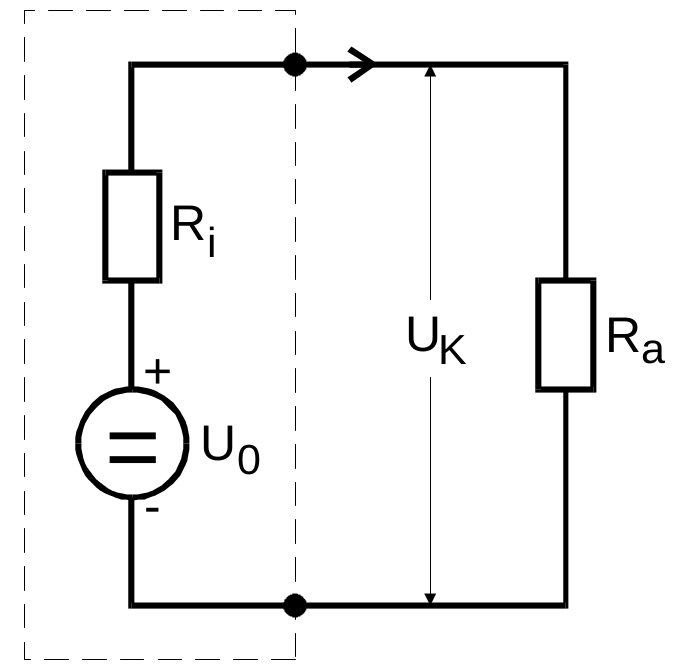
\includegraphics[width=0.4\textwidth]{pics/reell.png}
 \caption{Ersatzschaltbild einer realen Spannungsquelle mit Lastwiderstand $R_a ^{[1]}$}
 \label{pic_reell}
\end{figure}
Aus dem zweiten Kirchhhoffschen Gesetz, der Maschenregel, folgt für das Problem
\begin{align}
\nonumber
 \sum U_{0_n} &= \sum I_m R_m\\ 
 U_0 &= IR_i + IR_a,
\end{align}
woraus sich für die Klemmspannung ergibt
\begin{align}
 U_k = IR_a = U_0-IR_i.
 \label{eq_klemmspannung}
\end{align}
Um die Leerlaufspannung zu ermitteln, sollte idealerweise kein Strom durch das Messgerät mit dem Lastwiderstand $R_a$ fließen. Durch ein
hochohmiges Voltmeter ist dies erreichbar, womit sich \eqref{eq_klemmspannung} ergibt zu
\begin{align}
 U_0 \approx U_k
\end{align}

\subsection{Leistungsanpassung}
Aufgrund des Innenwiderstands existiert ein Maximum der entnehmbaren Leistung $P$, die am Verbraucher $R_a$ genutzt werden kann.
\begin{align}
 P = U_k I = R_a I^2
\end{align}
Aus \eqref{eq_klemmspannung} ergibt sich
\begin{align}
 P = \frac{U^2_0\cdot R_a}{(R_a+R_i)^2}
 \label{eq_leistung}
\end{align}
Um das Leistungsmaximum in Abhängigkeit des Lastwiderstands zu bestimmen, wird \eqref{eq_leistung} nach $R_a$ abgeleitet und die 
entstehende Gleichung 0 gleichgesetzt.
\begin{align}
 \nonumber
 \frac{\partial P}{\partial R_a} = \frac{U^2_0\,(R_a+R_i)-2U^2_0R_a}{(R_a+R_i)^3}&=0\\
 \nonumber
 U^2_0\,(R_a+R_i)-2U^2_0R_a&=0\\
 R_i &= R_a
\end{align}
Die Maximalleistung $P_{max}$ wird demnach erreicht, wenn der Innenwiderstand dem Lastwiderstand gleich ist. Der Wert lässt sich errechnen
durch 
\begin{align}
 P_{max} = \frac{U^2_0}{4R_i}.
 \label{eq_maxleistung}
\end{align}
Aufgrund des schlechten Wirkungsgrads der Leistungsanpassung wird sie in Starkstromtechnik nicht angewandt. Jedoch in der Signalübertragung
findet sie Gebrauch.

\section{Durchführung}
Im Verlauf des Experiments werden vier Messreihen zur Bestimmung des Innenwiderstands und der Leerlaufspannung vorgenommen, sowie eine
Direktmessung mittels eines Voltmeters.
\subsection{Monozelle}
\subsubsection{ohne Gegenspannung}
\label{sec_ogegen}
Entsprechend Schaltbild \ref{pic_ogegenspannung} werden ein regelbarer Widerstand im Bereich von 0-50 $\Omega$ und die Messgeräte aufgebaut.
\begin{figure}[H]
 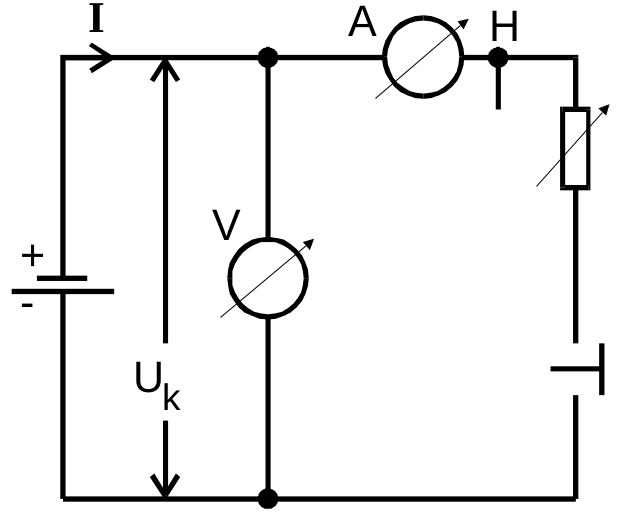
\includegraphics[width=0.5\textwidth]{pics/ohne.png}
 \caption{Versuchsaufbau für die Monozelle ohne Gegenspannung$^{[1]}$}
 \label{pic_ogegenspannung}
\end{figure}
Zu verschiedenen Widerständen im angegeben Bereich werden die Klemmspannungen $U_k$ mit den entsprechenden Strömen $I$ mit den entsprechenden
Messgeräten notiert.
\subsubsection{mit Gegenspannung}
Eine zweite Spannungsquelle wird nun gemäß Schaltbild \ref{pic_mgegenspannung} in den Verlauf integriert und die Messwerte identisch zu Abschnitt
\ref{sec_ogegen} aufgenommen.
\begin{figure}[H]
 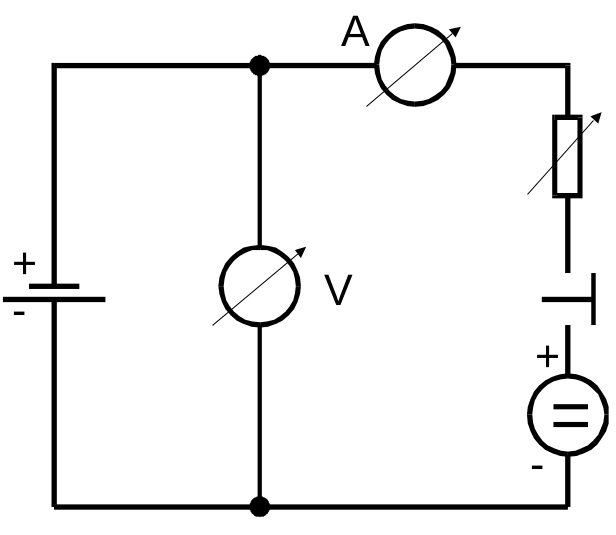
\includegraphics[width=0.5\textwidth]{pics/mit.png}
 \caption{Versuchsaufbau für die Monozelle mit Gegenspannung$^{[1]}$}
 \label{pic_mgegenspannung}
\end{figure}
\subsubsection{RC-Generator}
Hierbei wird die Monozelle durch einen RC-Generator ersetzt. Es wird je eine Messreihe ensprechend Abschnitt \ref{sec_ogegen} aufgenommen
für den Betrieb mit Rechtecksspannung mit dem regelbaren Widerstand im Bereich von 20-250 $\Ohm$, sowie mit Sinusspannung im Bereich von
0,1-5 k$\Ohm$.
\section{Auswertung}

\section{Diskussion}

% ========================================
%	Literaturverzeichnis
% ========================================

%\bibliographystyle{plainnat}			% Bibliographie-Style auswählen
%\bibliography{BIBDATEI}			% Literaturverzeichnis

% ========================================
%	Das Dokument endent
% ========================================

\end{document}
